\subsection{Pileup reweighting uncertainties}
As discussed in section~\ref{subsec:PRW}, a correction is applied to MC events such that the pileup modeling in the simulation corresponds to what is seen in data. As such, there are variations associated with this modeling
that must be taken into account.

In addition, a scaling correction is applied to the data during pileup reweighting. Nominally, this scaling correction is equal to 1/1.03, and the up and down variations are set to 1/1.072 and 1/1.35 respectively.

\subsection{Muon uncertainties}

\subsubsection{Muon efficiency uncertainties}
As summarized in section~\ref{subsec:MCCorr} there are several scale factors associated with muon reconstruction related to efficiencies in the trigger, reconstruction, isolation and track-to-vertex association.
Hence, there are 2 systematic variations associated with the trigger efficiency, 2 for the isolation efficiency, 4 for the reconstruction efficiency, and 2 for the TTVA efficiency:
\begin{itemize}
  \item MUON\_EFF\_TrigSystUncertainty
  \item MUON\_EFF\_TrigStatUncertainty
  \item MUON\_EFF\_ISO\_SYS
  \item MUON\_EFF\_ISO\_STAT
  \item MUON\_EFF\_RECO\_SYS
  \item MUON\_EFF\_RECO\_SYS\_LOWPT
  \item MUON\_EFF\_RECO\_STAT
  \item MUON\_EFF\_RECO\_STAT\_LOWPT
  \item MUON\_EFF\_TTVA\_SYS
  \item MUON\_EFF\_TTVA\_STAT
\end{itemize}

The impact of the efficiency systematics is summarized in figure~\ref{fig:PP8SFSyst}.

\begin{figure}[h!]
  \centering
  \subfloat[MC16a]{\includegraphics[page=2,width=\textwidth]{figures/ZjetOmnifoldSystematics.pdf}} \\
  \subfloat[MC16d]{\includegraphics[page=9,width=\textwidth]{figures/ZjetOmnifoldSystematics.pdf}} \\
  \subfloat[MC16e]{\includegraphics[page=16,width=\textwidth]{figures/ZjetOmnifoldSystematics.pdf}} \\
  \subfloat[Run 2]{\includegraphics[page=22,width=\textwidth]{figures/ZjetOmnifoldSystematics.pdf}}
  \caption{The fractional systematic impact for the pileup efficiency and the muon efficiencies for the \powheg+\pythia~samples across all years as a function of the dilepton \pt. The upwards shift is presented in red, and the downwards shift in blue.}
  \label{fig:PP8SFSyst}
\end{figure}

\subsubsection{Muon calibration uncertainties}
There are also systematic variations associated with the calibration applied to the muons. These will have an affect on the muon kinematics. The systematic variations are listed below, and include
one for momentum variations due to measurements made in the inner detector, one for momentum effects related to the muon spectrometer, one for the momentum scale, and 2 systematics related to the measured sagitta value.
\begin{itemize}
  \item MUON\_ID (inner detector track resolution)
  \item MUON\_MS (muon spectrometer track resolution)
  \item MUON\_SCALE (momentum scale)
  \item MUON\_SAGITTA\_RESBIAS (residual bias correction)
  \item MUON\_SAGITTA\_RHO (combined measurement correction)
\end{itemize}

The effects of these variations are shown in figure~\ref{fig:PP8MuCalSyst}.

\begin{figure}[h!]
  \centering
  \subfloat{\includegraphics[page=5,width=\textwidth]{figures/ZjetOmnifoldSystematics.pdf}} \\
  \subfloat{\includegraphics[page=12,width=\textwidth]{figures/ZjetOmnifoldSystematics.pdf}} \\
  \subfloat{\includegraphics[page=19,width=\textwidth]{figures/ZjetOmnifoldSystematics.pdf}} \\
  \subfloat{\includegraphics[page=25,width=\textwidth]{figures/ZjetOmnifoldSystematics.pdf}}
  \caption{The fractional systematic impact for variations to the muon calibration for the \powheg+\pythia~samples for all years as a function of the dilepton \pt. The upwards shift is presented in red, and the downwards shift in blue.}
  \label{fig:PP8MuCalSyst}
\end{figure}

\subsection{Track uncertainties}

The systematic uncertainties associated with the tracks are:

\begin{itemize}
  \item InDet::TRK\_EFF\_TIGHT\_GLOBAL
  \item InDet::TRK\_EFF\_TIGHT\_IBL
  \item InDet::TRK\_EFF\_TIGHT\_PP0
  \item InDet::TRK\_EFF\_TIGHT\_PHYSMODEL
  \item InDet::TRK\_EFF\_LOOSE\_TIDE
  \item InDet::TRK\_FAKE\_RATE\_LOOSE
  \item InDet::TRK\_BIAS\_QOVERP\_SAGITTA\_WM
\end{itemize}

The first four are combined into one nuisance parameter and are due to variations of the tracking efficiency. The fifth describes the variations to the tracking efficiency when the track is inside a jet.
The sixth represents variations to the fake rate. The last varies the \pt of the track based on the residual alignment uncertainties.

\begin{figure}[h!]
  \centering
  \subfloat[MC16a]{\includegraphics[page=7,width=0.45\textwidth]{figures/ZjetOmnifoldSystematics.pdf}}
  \subfloat[MC16d]{\includegraphics[page=14,width=0.45\textwidth]{figures/ZjetOmnifoldSystematics.pdf}} \\
  \subfloat[MC16e]{\includegraphics[page=21,width=0.45\textwidth]{figures/ZjetOmnifoldSystematics.pdf}}
  \subfloat[Run 2]{\includegraphics[page=27,width=0.45\textwidth]{figures/ZjetOmnifoldSystematics.pdf}}
  \caption{The fractional systematic impact for variations applied to the tracks for the \powheg+\pythia~samples for all years. Note that only the down variations are shown for the inclusive efficiency, inside jet efficiency and the fake rate.
  The variations are symmetrized for use in the analysis.}
  \label{fig:PP8TrackSyst}
\end{figure}

\subsection{Modeling and unfolding uncertainties}
